%\documentclass[handout]{beamer}
\documentclass{beamer}
\mode<article>
{
	\usepackage{amscd}
	\usepackage{times,amsmath,amsbsy,amssymb,amsfonts,epic,hyperref}
	\usepackage[pdftex]{geometry}
	\usepackage[pdftex]{graphicx}
	\usepackage{fullpage}
	\usepackage{hyperref}
}

%\mode<presentation> {
%\usetheme{Madrid}
%\usecolortheme{dolphin}
%\usecolortheme{rose}
%}
\usepackage{amsfonts,bm,mathrsfs,subfig}
%\usepackage{movie15}

\mode<presentation> {
	\setbeamertemplate{background canvas}[vertical shading][bottom=red!10,top=blue!10]
	\usetheme{Boadilla}
	\usefonttheme[onlysmall]{structurebold}
}

\usepackage{multimedia}
\usepackage{animate} %need the animate.sty file

\usepackage{pgf,pgfarrows,pgfnodes,pgfautomata,pgfheaps,pgfshade,multirow}
\usepackage{amscd}
\usepackage{amsmath,amssymb}
%\usepackage[latin1]{inputenc}
\usepackage{colortbl}
\usepackage[english]{babel}
\usepackage{times}
\usepackage[T1]{fontenc}
\usepackage{epsf}
\usepackage{epsfig}
\usepackage{graphicx}
\usepackage{bm}
\usepackage{relsize}
\usepackage{dsfont}
\usepackage{pifont}
\usepackage{comment}
\usepackage{booktabs}
\newtheorem{algorithm}{Algorithm}
\newtheorem{remark}{Remark}
\usepackage{undertilde}
\usepackage{fancybox}
\usepackage{CJK}
\usepackage{multirow}
\usepackage{tikz}
\usepackage{slashbox}

%\input{mydef}
\def\p{\partial}
\def\u{{\mathbf u}}
% \def\B{{\mathbf B}}
\def\v{{\mathbf v}}
\def\n{{\mathbf n}}
% \def\F{{\mathbf F}}
%\def\A{{\mathbf A}}
% \def\x{{\mathbf x}}
\def\DD{\displaystyle}

\newcommand*{\ucong}{\mathrel{\text{\raisebox{.25ex}{\rotatebox[origin=c]{180}{$\cong$}}}}}
\newcommand{\relu}{\mbox{{\rm ReLU}}}



\newcommand{\red}[1]{\textcolor{red}{#1}}
\newcommand{\blue}[1]{\textcolor{blue}{#1}}
\newcommand{\brown}[1]{\textcolor{brown}{#1}}
\newcommand{\green}[1]{\textcolor{green}{#1}}


\newtheorem{prop}{Proposition}
\newtheorem{thm}{Theorem}
\newtheorem{prob}{Problem}
\newtheorem{assumption}{Assumption}
\newtheorem{defn}{Definition}
\newtheorem{coro}{Corollary}
\beamertemplatenavigationsymbolsempty


\newcommand{\tabincell}[2]{\begin{tabular}{@{}#1@{}}#2\end{tabular}}  

\newif\iflattersubsect

\AtBeginSection[] {
	\begin{frame}<beamer>
	\frametitle{Outline} %
	\tableofcontents[currentsection]  
\end{frame}
\lattersubsectfalse
}

\AtBeginSubsection[] {
\iflattersubsect
\begin{frame}<beamer>
\frametitle{Outline} %
\tableofcontents[currentsubsection]  
\end{frame}
\fi
\lattersubsecttrue
}

\begin{document}

\begin{CJK*}{UTF8}{gbsn}


\title
{Deep Learning}

\author[Jinchao Xu]{Jinchao Xu}

\institute[PSU]
{Penn State University\\[0.2cm]
	
}

\date{Jan 8, 2019}

\begin{frame}
\titlepage


\end{frame}


\begin{frame}\frametitle{Course info} 
\begin{description}
\item[Instructor] Professor Jinchao Xu, 314 McAllister Building, {\color{blue}\tt xu@math.psu.edu }, {\color{blue}\tt http://www.math.psu.edu/xu/}
\item[Time] Tuesday and Thursday 12:05pm-1:20pm, 114 McAllister Building
\item[Office hours:] Tuesday and Thursday 3:00pm-4:00pm
\item[PREREQUISITE:]
A good knowledge of multi-variable calculus, linear
algebra and basic numerical analysis

\item[REQUIREMENT:  ]$\quad$

  \begin{itemize}
  \item Homework and programming assignments  (60\%) 
\item Take-Home Midterm (20\%) Take-Home Final (20\%).
  \end{itemize}
\item[REFERENCES:]  PDF files of detailed lectures notes will be available to
the  class.
\end{description}

\end{frame}




\begin{frame}
{Topics}
\begin{itemize}
\item Elements of probability and statistics
\item Basic theory of machine learning
\item Basic structure of deep neural networks
\item Approximation properties of DNN 
\item Convolutional neural networks
\item Recurrent neural networks
\item Generative Adversarial Networks
\item Stochastic gradient descent methods 
\item DNN and finite element methods
\item Multigrid methods
\item MgNet
\item Python
\item MNIST
\item TensorFlow, PyTorch
\end{itemize}
\end{frame}


\begin{frame}
\frametitle{Four major methods of scientific research}
\begin{columns}
	\begin{column}{0.5\textwidth}
		\centering
		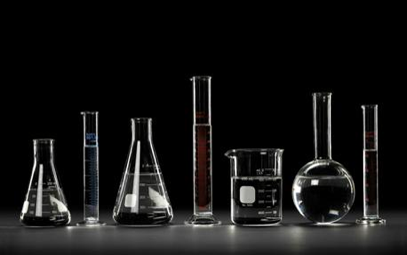
\includegraphics[width=0.8\linewidth]{figures/Experimental} \\
		Experimental Science
		\vspace{4mm}
		
		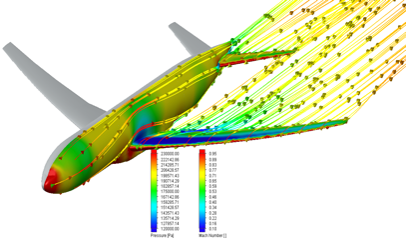
\includegraphics[width=0.8\linewidth]{figures/Computational} \\
		Computational Science
	\end{column}
	
	\begin{column}{0.5\textwidth}
		\centering
		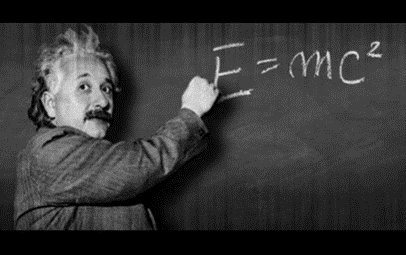
\includegraphics[width=0.8\linewidth]{figures/Theoretical.png} \\
		Theoretical Science
		
		\vspace{4mm}
		
		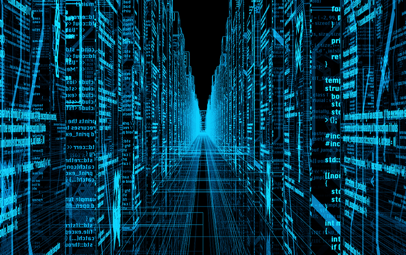
\includegraphics[width=0.8\linewidth]{figures/Data.png} \\
		Data Science
	\end{column}
\end{columns}
\end{frame}

\begin{frame}
\frametitle{The era of the artificial intelligence}
		\centering
		\includegraphics[width=0.8\linewidth]{figures/aiera} 
\end{frame}

\begin{frame}{Example: different approaches to language learning}
\begin{itemize}
	\item Non-Native speakers (more a theoretical approach )
	\begin{itemize}
	\item Rules of pronunciation,  syntax, ...
	\end{itemize}
    \item Native speakers (more a data approach )
	\begin{itemize}
	\item Imitating ...
	\end{itemize}
Which one is more scientific or more effective?
\end{itemize}
\end{frame}



\begin{frame}{A basic AI problem: classification}
\begin{itemize}
	\item Can a machine (function) tell the difference ?
\end{itemize}
\begin{figure}
	\begin{center}
		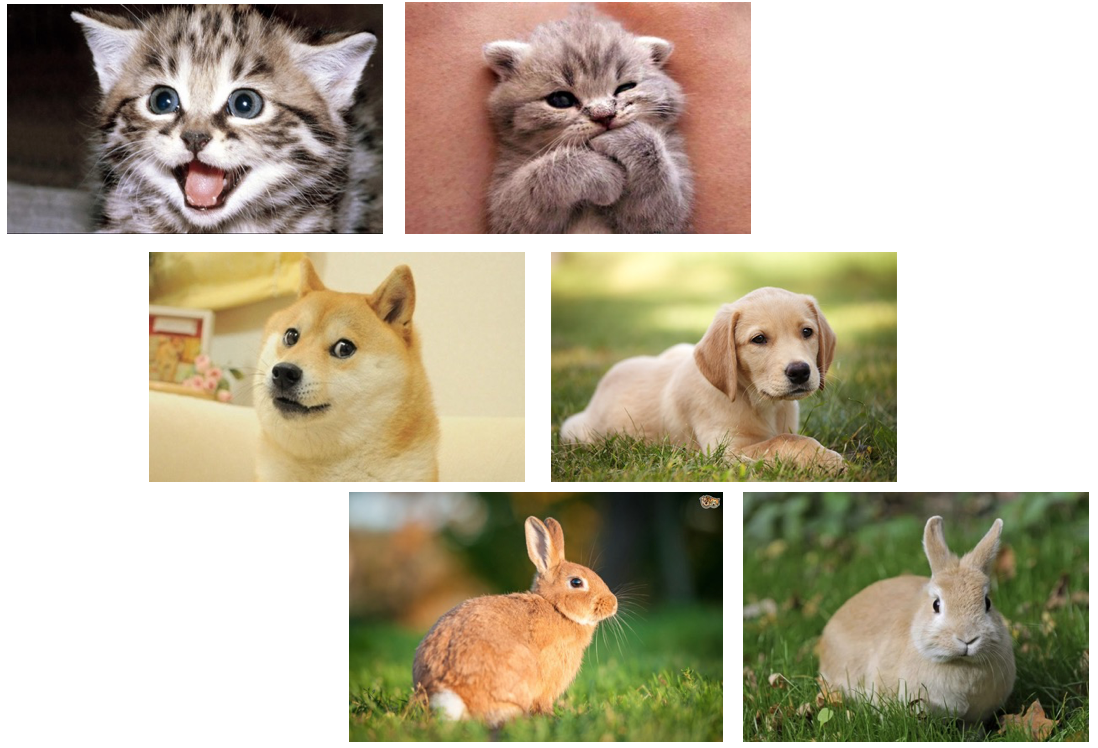
\includegraphics[width=.7\textwidth, height=.6\textheight]{figures/cat-dog-1.png} 
	\end{center}
\end{figure}

\end{frame}

\begin{frame}{Supervised learning $\leftrightarrow$ Function interpolation}
\begin{itemize}
\item Each image = a big vector of pixel values 
\begin{itemize}
	\item $n=1280\times720\times3$ (width$\times$ height $\times$ RGB channel) $\approx$ 3M. 
\end{itemize}

\item 3 different sets of points in $\mathbb{R}^n$, are they separable?
\begin{figure}
	\begin{center}
		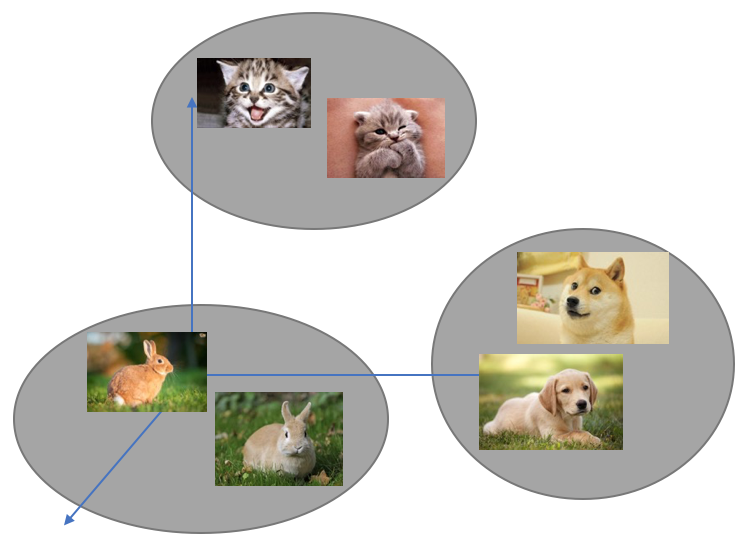
\includegraphics[width=.3\textwidth, height=.3\textheight]{figures/cat-dog-2.png}   \quad \quad  \quad \quad 
		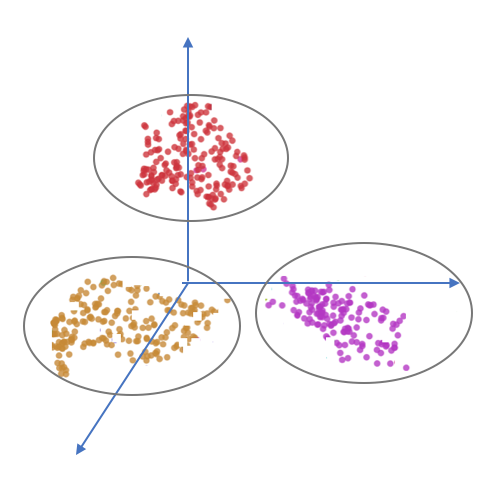
\includegraphics[width=.3\textwidth, height=.3\textheight]{figures/cat-dog-3.png}  
	\end{center} 
\end{figure}
\item Mathematical problem: Find $f(\cdot; \Theta): \mathbb{R}^n \to \mathbb{R}^3$ such that:
$$
f(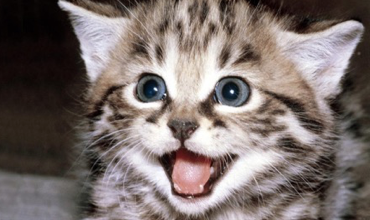
\includegraphics[width=.07\textwidth]{figures/cat.png}; \Theta)
\approx \begin{pmatrix}
1\\ 0 \\ 0 
\end{pmatrix} 
\quad 
f(
\includegraphics[width=.07\textwidth]{figures/dog.png}; \Theta)
\approx \begin{pmatrix}
0\\ 1 \\ 0 
\end{pmatrix} 
\quad 
f(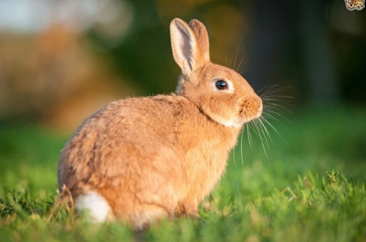
\includegraphics[width=.07\textwidth]{figures/rabbit.png};
    \Theta) \approx 
\begin{pmatrix}
0\\ 0 \\ 1
\end{pmatrix} 
$$
\end{itemize}
\end{frame}

\begin{frame}{One core problem of AI: clustering}
One simple example
\begin{itemize}
	\item A collection of points $\mathbb{R}^{N}$ is separated into several classes somehow ...
    \item The object is to construct a function y=f(x). The input x of the function is the coordinated of the points in the space and the output y is the cluster the point belongs to.
	\begin{center}
		\includegraphics[width=.35\textwidth]{figures/dots} 
	\end{center}
\end{itemize}
\end{frame}



\begin{frame}{Graph Recognition}
\begin{columns}
\begin{column}{0.6\textwidth}
\begin{itemize}
\item In 1998, LeCun etc. proposed the neural network LeNet-5 based on the convolution and applied to the hand-written digits recognition successfully. Hence LeNet-5 is also called the first convolutional neural network(CNN) successfully applied.

\item In 2012, Hinton and his student Alex joined the graph recognition competition by ImageNet and improved the accuracy significantly with the CNN AlexNet.

\item Afterwards CNN is widely used in the field of computer vision and breaks the records ceaselessly.

\end{itemize}
\end{column}

\begin{column}{0.4\textwidth}
\centering  
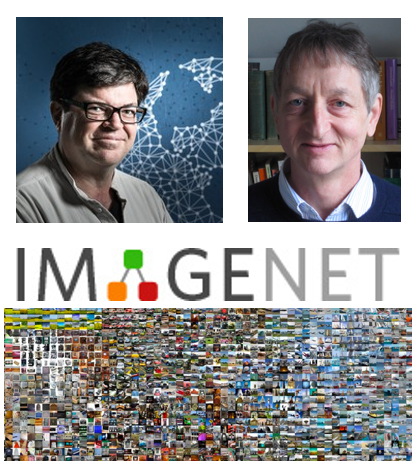
\includegraphics[width=\textwidth]{figures/ImageNet}  \\
%\centering  
%\includegraphics[width=\textwidth, height= 0.4\textheight]{figures/Alphago}  
\end{column}

\end{columns}
\end{frame}



\begin{frame}{AlphaGo $\&$ AlphaZero}
One simple example
\begin{itemize}
	\item From 2016 to 2017, the AI program AlphaGo developed by Google DeepMind beat down all the Go champions worldwide. 

    \item 2018 AlphaZero gave a unified principle for many other board games.
    \item The CEO of Google DeepMind Demis Hassabis announced to integrate AlphaGo with medical, robots and so on. They can learn by themselves since they are artificial intelligence, and transfer learning can be done with enough data.
\end{itemize}

	\begin{center}
		\includegraphics[width=.5\textwidth]{figures/Alphago2} 
	\end{center}
\end{frame}


\begin{frame}{Auto-driving (the next competition in AI)}
\begin{columns}
\begin{column}{0.6\textwidth}
\begin{itemize}
\item In 2009, Google proposed the plan to replace human driving with softwares.

\item Afterwards, many large technology companies such as Tesla, Google, Uber and Benz devoted a lot on investigating the technology of automated driving.

\item In many countries, road examination autonomous vehicles are allowed with applications.

\item In China, Baidu established the division of intelligent car and opened the platform of automated driving to the public.

\end{itemize}
\end{column}

\begin{column}{0.4\textwidth}
\centering  
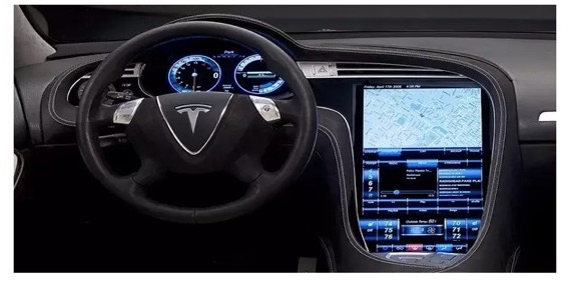
\includegraphics[width=\textwidth]{figures/AutomatedDriving1}  \\
\centering  
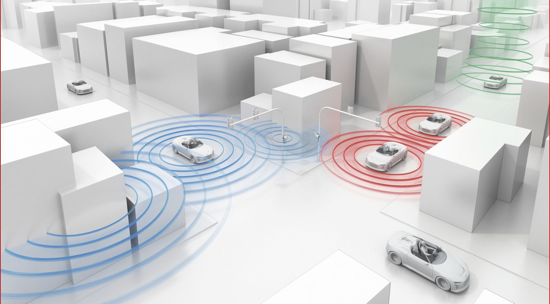
\includegraphics[width=\textwidth]{figures/AutomatedDriving2}  
\end{column}
\end{columns}
\end{frame}


\begin{frame}{Speech recognition}
\begin{columns}
\begin{column}{0.6\textwidth}
\begin{itemize}
\item Recently, the application of recurrent neural network(RNN) and attention model on the speech recognition has achieved great breakthrough on the accuracy of AI speech recognition.

\item On October 18 2016, during the Smartisan mobile phone launch event, the input speed of iFLY surpassed that of the real keyboards and achieved 100\% in accuracy.

\item In Nov 2016, IFLYTEK, Baidu, Sogou announced they achieved 97\% in the accuracy of Chinese speech recognition respectively.


\item 2018, Google propose the BERT as a evolutionary model in NLP field.
\end{itemize}
\end{column}

\begin{column}{0.4\textwidth}
\centering  
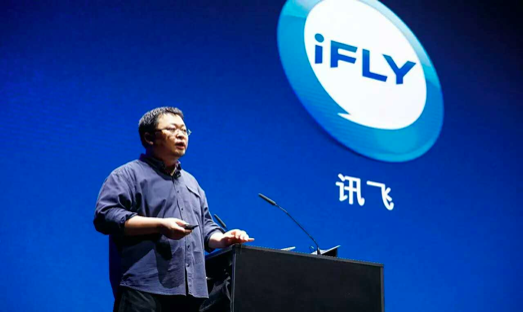
\includegraphics[width=\textwidth]{figures/SpeechRecognition1}  \\
\centering  
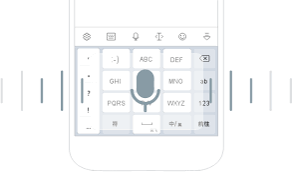
\includegraphics[width=\textwidth]{figures/SpeechRecognition2}  
\end{column}
\end{columns}
\end{frame}


\begin{frame}{Machine translation}
\begin{columns}
\begin{column}{0.6\textwidth}
\begin{itemize}
\item On Sep 27 2016,  Google posed a paper in ArXiv.org about Google's Neural Machine Translation (GNMT). On 28th, to the extremely difficult Chinese-English translation. 

\item 2018, Baidu, Microsoft, Google announced that they proposed some model to translate better than humans in some certain fields and languages.
\end{itemize}
\end{column}

\begin{column}{0.4\textwidth}
\centering  
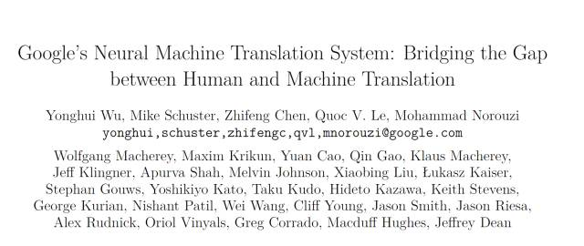
\includegraphics[width=\textwidth]{figures/MachineTranslation1}  \\
\centering  
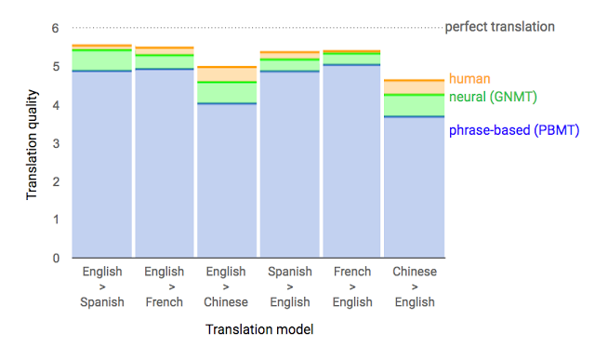
\includegraphics[width=\textwidth]{figures/MachineTranslation2}  
\end{column}
\end{columns}
\end{frame}


\begin{frame}{Future smart healthcare}
\begin{columns}
\begin{column}{0.6\textwidth}
\begin{itemize}
\item In 2015, Watson diagnosed leukemia for a 60-year old woman within 10 minutes and proposed adequate therapeutic schedule to Institute of medical science, University of Tokyo

\item On the world cancer day in 2017, Watson wrote a prescription for a patient with advanced gastric cancer within 10 seconds in Tianjin third central hospital

\item The future scope of the big data on medical and smart healthcare is broad. 
\end{itemize}
\end{column}

\begin{column}{0.4\textwidth}
\centering  

\includegraphics[width=\textwidth]{figures/Watson1}  \\
\centering  
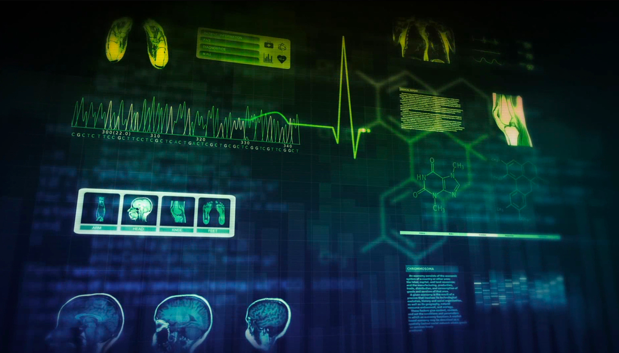
\includegraphics[width=\textwidth]{figures/Watson2}  
\end{column}
\end{columns}
\end{frame}


\begin{frame}{Artificial intelligent}
\centering  
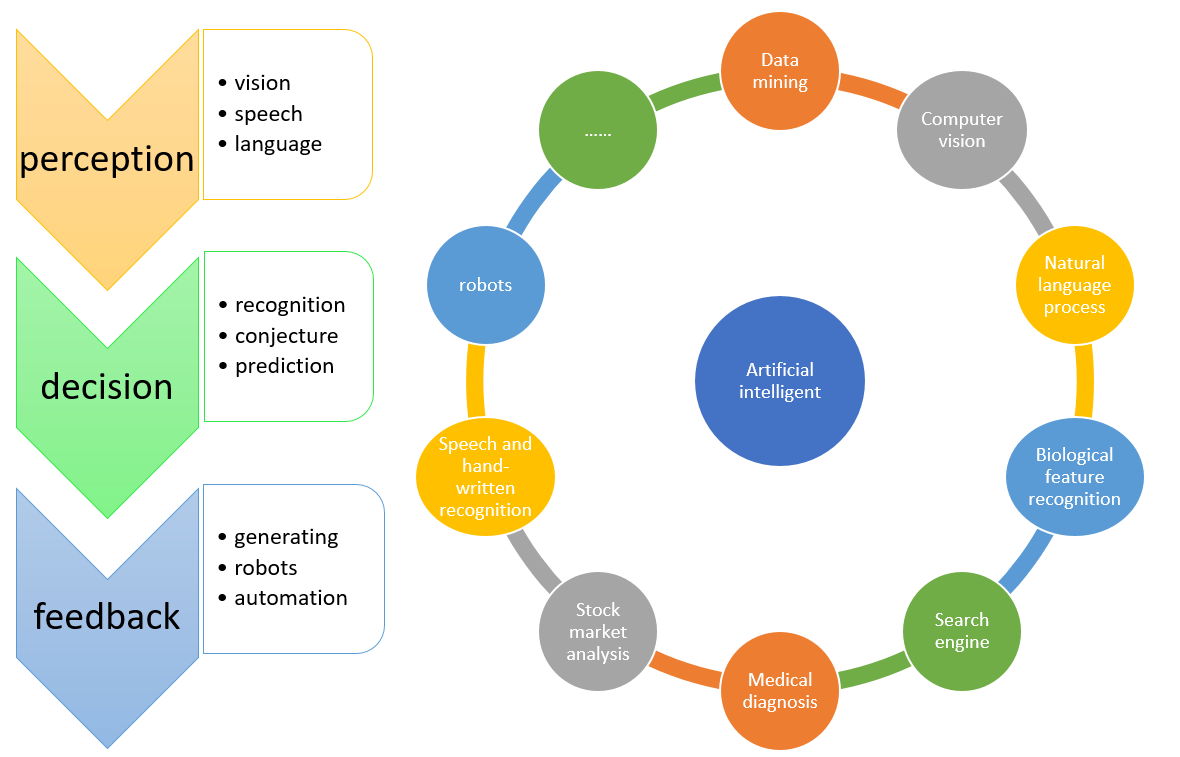
\includegraphics[width=.8\textwidth]{figures/AI}
\end{frame}


\begin{frame}{Machine learning}
\centering  
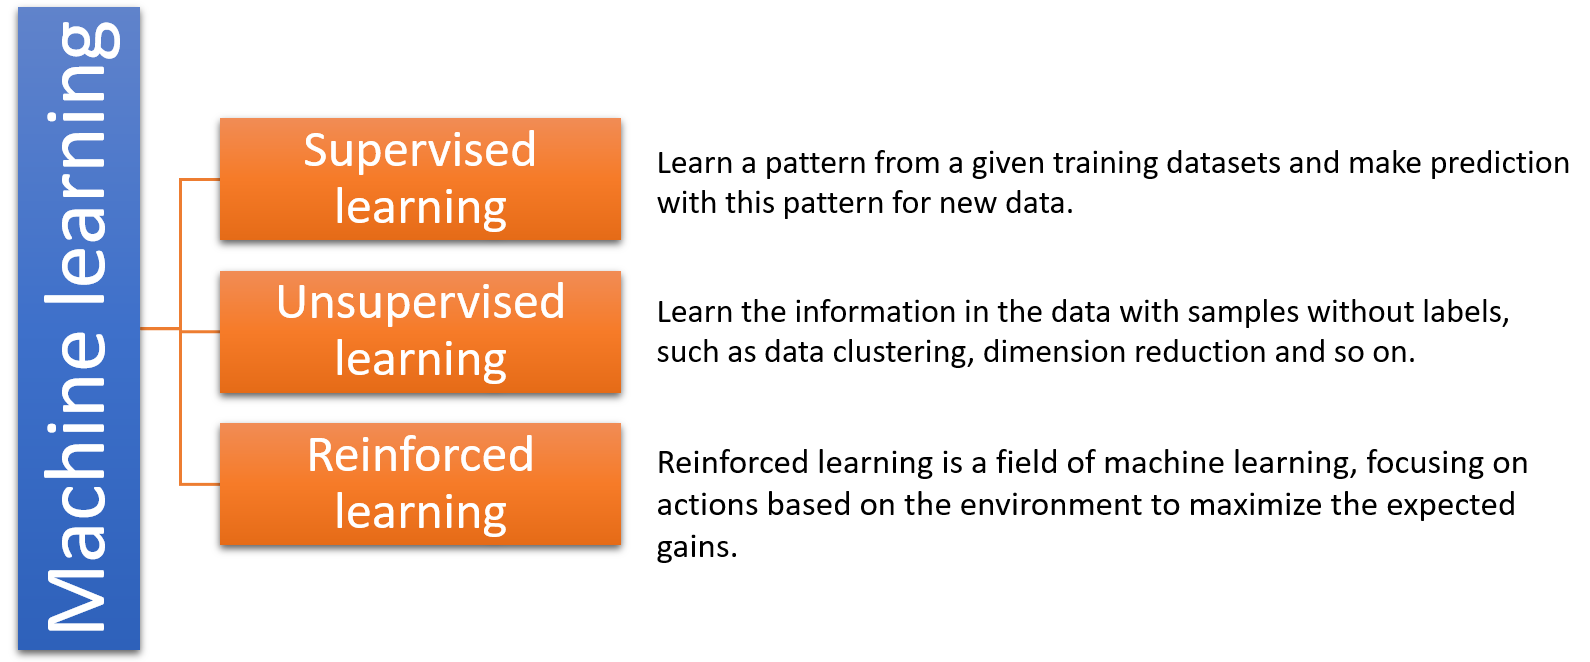
\includegraphics[width=.8\textwidth]{figures/ML}
\end{frame}


\begin{frame}{Deep learning}
\centering  
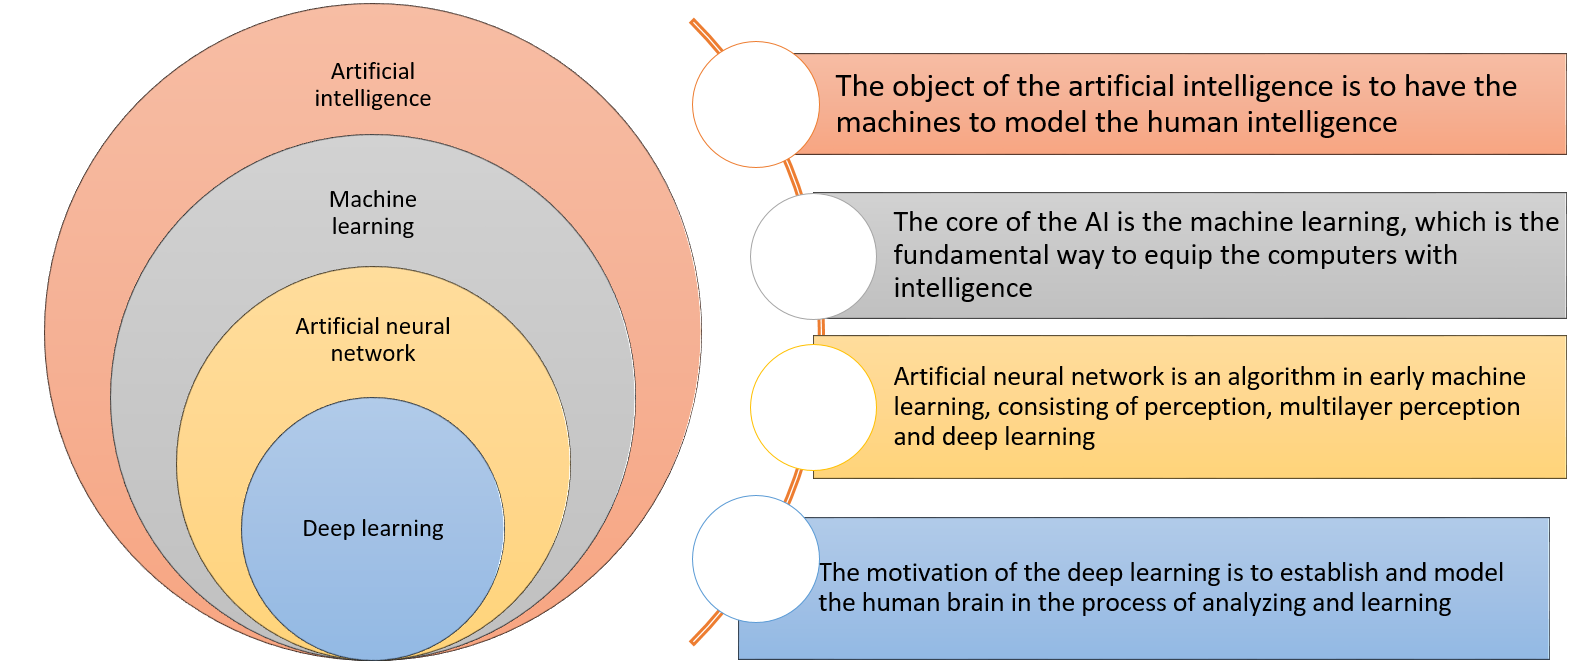
\includegraphics[width=.8\textwidth]{figures/DL}
\end{frame}


\begin{frame}{Neurons of animals}

\begin{itemize}
\item Dendrite: receive the electric signal from other neurons

\item Cell body: process the electric signal from other neurons

\item Axon: send the electric signal to other neurons

\item Activation: the intensity of the signal is larger than the threshold 


\end{itemize}
\begin{center}
\includegraphics[width=0.6\textwidth]{figures/cell}
\end{center}
\end{frame}


\begin{frame}{Artificial neuron}

\begin{itemize}
\item An artificial neuron consists of
\begin{itemize}
\item An affine transformation:  g(x)=Wx+b

\item A nonlinear function(activation fuction): $\phi$
\end{itemize}
\item The output of the neuron is $y=\phi(g(x))$

\end{itemize}
\begin{center}
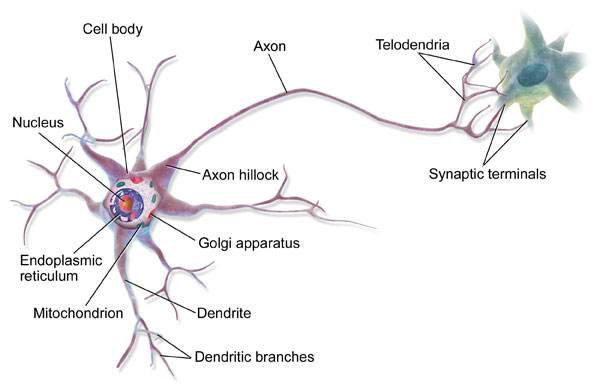
\includegraphics[width=0.6\textwidth]{figures/neuron}
\end{center}
\end{frame}


\begin{frame}{Major models in deep learning}
\centering  
\includegraphics[width=0.9\textwidth]{figures/models}
\end{frame}




\begin{frame}{Basic CNN model structure}
\begin{center}
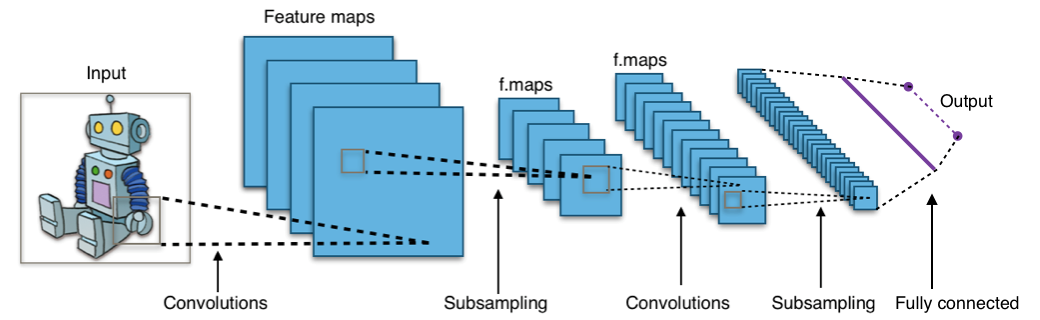
\includegraphics[width=0.8\textwidth]{figures/CNNPic}
\end{center}
\begin{itemize}
\item General convolutional neural network consists of:
\begin{itemize}
\item Convolution layers
\item Nonlinear layers(activation function)
\item Pooling layers
\item Fully-connected layers

\end{itemize}
\end{itemize}
\end{frame}


\begin{frame}{Convolution layer}
\begin{tabular}{cc}
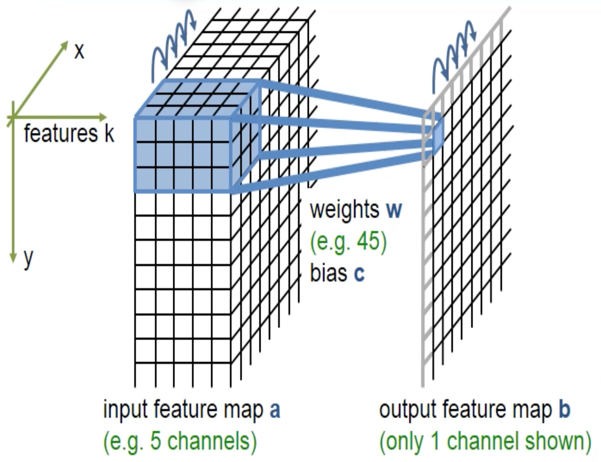
\includegraphics[width=0.45\textwidth]{figures/CNNLayer1} & 
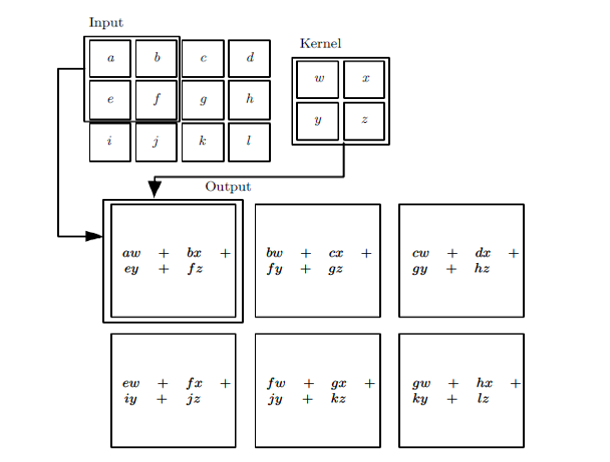
\includegraphics[width=0.45\textwidth]{figures/CNNLayer2}
\end{tabular}
\end{frame}


\begin{frame}{Convolutional kernel}
\begin{columns}
\begin{column}{0.4\textwidth}
\begin{itemize}
\item A convolutional layer consists of multiple convolutional kernel 
\item Each convolutional kernel extract a certain feature/channel
\item The graph processed after convolutional layer is called feature mapping
\end{itemize}
\end{column}

\begin{column}{0.6\textwidth}
\centering  
\includegraphics[width=\textwidth]{figures/kernel} 
\end{column}
\end{columns}
\end{frame}


\begin{frame}{Activation function}
\centering  
\includegraphics[width=0.9\textwidth]{figures/activate}
\end{frame}





\begin{frame}{Pooling layer}
\begin{columns}
\begin{column}{0.5\textwidth}
\begin{center}
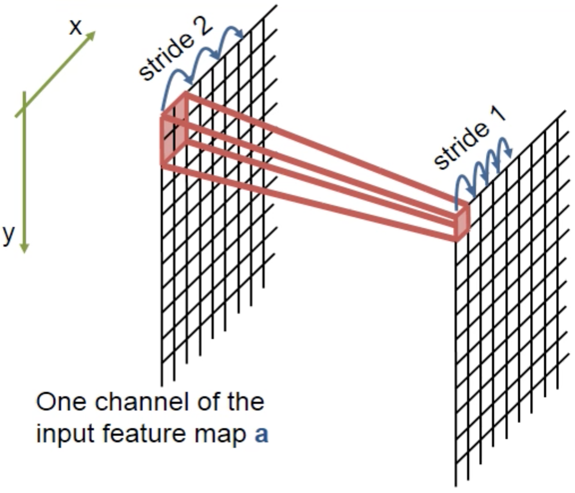
\includegraphics[width=.6\textwidth, height=0.4\textheight]{figures/PoolingLayer1} 
\end{center}

\end{column}
\begin{column}{0.5\textwidth}	
\begin{center}
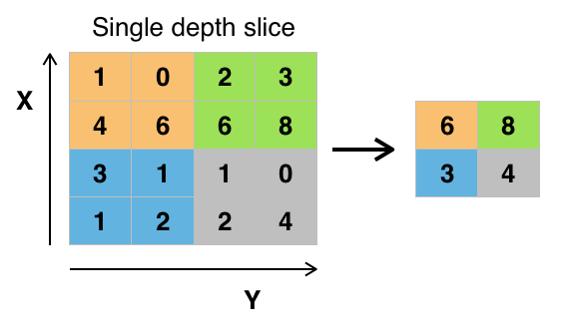
\includegraphics[width=.6\textwidth, height=0.4\textheight]{figures/PoolingLayer2}
\end{center}	

\end{column}
\end{columns}
\end{frame}


\begin{frame}{Fully-connected layers (DNN)}
\begin{columns}
\column{0.3\textwidth}  
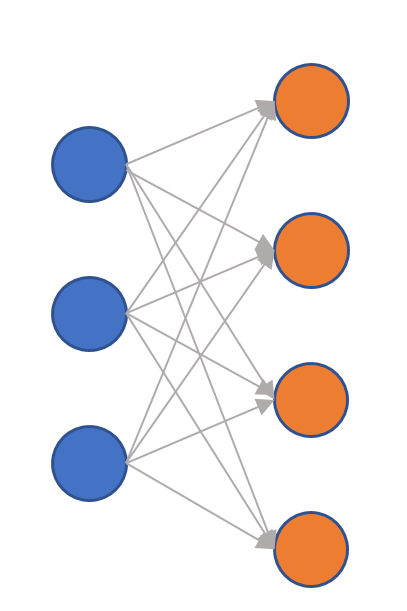
\includegraphics[width=\textwidth]{figures/FC}
\column{0.7\textwidth} % remember add this to the other clumn  
\begin{minipage}[c][0.45\textheight][c]{\linewidth} 
\begin{itemize}
\item Each neuron in the previous layer is connected with each neuron in the latter layer 
\item A fully-connected layer can be represented with the following linear function
$$y=Wx+b$$
\begin{itemize}
\item $x$ --- input
\item $y$ --- output
\item $W,b$--- parameters

\end{itemize}
\item Fully-connected layer makes classification with the features extracted by the convolutional layer

\end{itemize}

\end{minipage}
\end{columns}  
\end{frame}

\begin{frame}
  \frametitle{A typical machine learning process}
  \begin{enumerate}
  \item Dimension reduction (linear or nonlinear)
    \begin{itemize}
    \item Convolutional Neural Networks (CNN)
    \end{itemize}
\item Classifier (linear)
  \begin{itemize}
  \item Fully connected layer
  \end{itemize}
  \end{enumerate}
  \begin{center}
		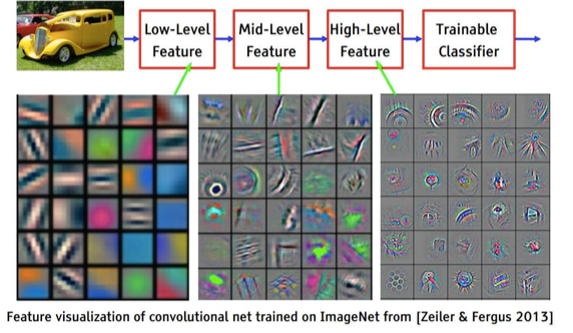
\includegraphics[width=.5\textwidth]{figures/CNNKernel}    
  \end{center}
\end{frame}

\begin{frame}{A complete convolutional neural network example}
\begin{columns}
\column{0.25\textwidth}  
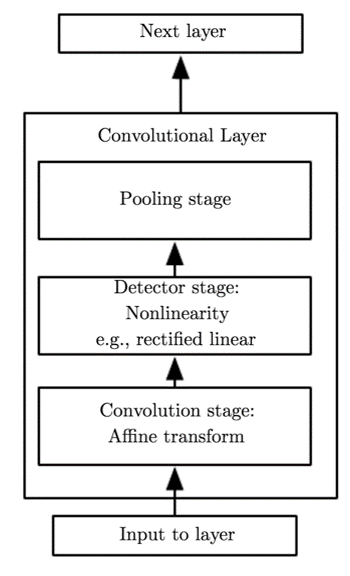
\includegraphics[width=\textwidth]{figures/CNN1}
\column{0.7\textwidth} % remember add this to the other clumn  
\begin{figure}
\begin{center} 
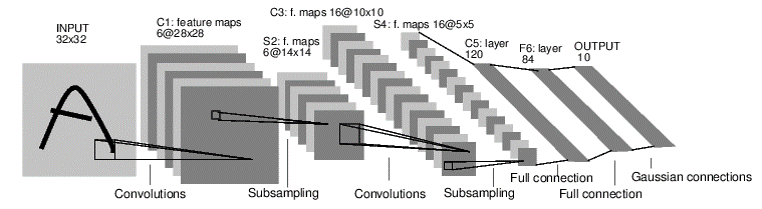
\includegraphics[width=\linewidth]{figures/CNN2}  
\caption{First convolutional neural network: LeNet-5 (Y. LeCun, L. Bottou, Y. Bengio, and P. Haffner, 1998)}
\end{center}
\end{figure} 
\begin{itemize}
\item Convolutional layer: extract the features of the graphs 
\item Fully-connected layer: make classification with the extracted features
\end{itemize}
\end{columns}  
\end{frame}



\begin{frame}{An example of convolutional neural network: AlphaGo}
\centering  
\includegraphics[width=0.9\textwidth]{figures/Alphago3}
\end{frame}


\begin{frame}{Deep convolutional neural network}
\centering  
\includegraphics[width=0.9\textwidth]{figures/deepcnn}
\end{frame}



\begin{frame}{Learning(training)}
The process of learning is the process to minimize the loss function 
$\min_{W\in \mathbb{R}^n}\frac{1}{m}\Sigma^m_{i=1}L(f(X^i;W),Y^i)$

\begin{itemize}
\item Training methods in common use: gradient descend, stochastic gradient descend, simulating annealing, etc.

\item The training time is extremely long for the current deep neural network due to the plentiful parameters. It takes several weeks to train a traditional deep learning model
    \begin{itemize}
\item AlexNet: takes 5-6 days to train on two GTX 580 3GB GPU
\item VGGNet: takes 2-3 weeks to train on NVIDIA Titan Black GPU
\item ResNet-50: 30 hours on DGX-1, 224 seconds on (Nvidia V100*2176 ≈ \$ 13M)
\end{itemize}
\item Research direction:improvement on the models and training algorithms
\begin{itemize}
\item Construct more efficient neural network model: deep or shallow?

\item Implement efficient and stable training algorithms

\item GPU? TPU? Or CPU only?
\end{itemize}
\end{itemize}
\end{frame}


\begin{frame}{Medical AI - I }
\begin{columns}
\begin{column}{0.5\textwidth}
\begin{itemize}
\item Images  
\begin{itemize}
\item Medical images screening
\item Image registration
\item Organ segmentation in images
\item Diseased region extraction
\item Lesion feature classification
\end{itemize}

\item Biological parameters
\begin{itemize}
\item Disease diagnosis or alert based on the blood glucose, heart rate, ECG, etc.
\item Noninvasive detection of biological parameters such as blood glucose and blood fat
\end{itemize}

\item others
\begin{itemize}
\item Operation result prediction
\item Online medical
\end{itemize}

\end{itemize}
\end{column}

\begin{column}{0.5\textwidth}
\centering  
\includegraphics[width=\textwidth]{figures/aimedical} 
\end{column}
\end{columns}
\end{frame}




\begin{frame}{Medical AI - II}
\begin{itemize}
\item 1970s --- 1990s: traditional methods: manual set rules + mathematical modeling 
\item 1990s --- 2000s: manual feature extraction+ supervised learning
\item 2000s --- 2010s:  end to end(automatic feature extraction+ learning)
\end{itemize}
\begin{center}
\includegraphics[width=0.8\textwidth]{figures/medicalai}
\end{center}
\end{frame}


\begin{frame}{Medical AI - III}
AI can automatically diagnose the cancer
\begin{itemize}
\item In 2017,  a team in Stanford University achieved AI automatic diagnosis of the skin cancer with the CNN, the accuracy of which is as high as a human expert.
\item This model is trained based on a public model  by Google, while the original model is only used to classify the cats and dogs in photos.
\end{itemize}
\begin{center}
\includegraphics[width=0.8\textwidth]{figures/medicalai1}
\end{center}
\end{frame}


\begin{frame}{Medical AI - IV}
The deep neural network has achieved the recognition of focus position in medical images:
\begin{itemize}
\item During 2016 to 2017,two famous data competition platforms Kaggle and Ali yuntianchi held competitions of pulmonary nodules intelligent diagnosis based on the CT images
\item The winner team used the U-Net model based on the CNN and achieved high accuracy
\end{itemize}
\begin{center}
\includegraphics[width=0.8\textwidth]{figures/medicalai2}
\end{center}
\end{frame}


\begin{frame}{Medical AI - V}
AI can generate the diagnosis report automatically
\begin{itemize}
\item By combining CNN and RNN, learned with X-Ray images of chest and corresponding diagnosis report data, it can be achieved for classification of chest X-Ray and generate the diagnosis report automatically
\end{itemize}
\begin{center}
\includegraphics[width=0.8\textwidth]{figures/medicalai3}
\end{center}
\end{frame}


\begin{frame}{Generative Adversarial Networks}
\centering  
\includegraphics[width=0.9\textwidth]{figures/gan}
\end{frame}


\begin{frame}{GAN: similar to word embedding 
}
\centering  
\includegraphics[width=0.9\textwidth]{figures/gan2}
\end{frame}


\begin{frame}{Text to Image, by conditional GAN}
\centering  
\includegraphics[width=0.9\textwidth]{figures/gan3}
\end{frame}



\begin{frame}{Text to Image, by conditional GAN}
\centering  
\includegraphics[width=0.9\textwidth]{figures/gan4}
\end{frame}










\begin{frame}
\frametitle{2019-summer undergraduate course}
\begin{center}
\includegraphics[width=0.45\linewidth]{figures/flyer.pdf}
\end{center}
\end{frame}





\end{CJK*}
\end{document}


